\begingroup
\renewcommand\thechapter{A}
{\normalfont\huge\bfseries}{}{}{\Huge}
\chapter{Appendix}
\section{Command Line Utilities} \label{sec:appendix_user_guide}

The provided shell supports a variety of built-in commands. The \texttt{help} built-in provides a great starting point for exploring this functionality. We outline the provided functionality in Listing \ref{listing:app_help}.
 % \renewcommand{\ttdefault}{pcr}
\begin{lstlisting}[style=ShellInputStyle, deletekeywords={run, command, wc, echo, builtin, alias, return, in, ps, kill, help, exit, pwd, cd, cat, tee, time, false, true, test, set}, basicstyle=\tiny\ttfamily\color{shell_default}, label={listing:app_help}, caption={The \texttt{help} built-in provides a list of available commands}]
 +~$+ !help!
 Basic Commands
   §man§            display a manual pages                               @[builtin]@
   §echo§           writes the first argument to standard output         @[alias]@
   §led§            turns the LED on/off                                 @[builtin]@
   §run_memtest§    runs a memtest in a user-level thread                @[builtin]@
   §oncore§         run an application on a specific core                @[builtin]@
   §run§            run an application with the given command line       @[builtin]@
   §ps§             show the currently running processes                 @[builtin]@
   §kill§           kills the process with the specified pid             @[builtin]@
   §pause§          pauses the process with the specified pid            @[builtin]@
   §resume§         resumes the process with the specified pid           @[builtin]@
   §help§           show the available commands                          @[builtin]@
   §exit§           exits the active shell session                       @[builtin]@
 File Management Commands
   §pwd§            return working directory name                        @[builtin]@
   §cd§             change the working directory                         @[builtin]@
   §ls§             list directory contents                              @[alias]@
   §cat§            concatenate and print files                          @[alias]@
   §tee§            duplicate standard input                             @[alias]@
   §mkdir§          make directories                                     @[builtin]@
   §rmdir§          remove directories                                   @[builtin]@
   §rm§             remove directory entries                             @[builtin]@
Network Commands
  §ping§           ping IP address                                       @[alias]@
  §send§           send UDP packet                                       @[builtin]@
  §listen§         listen on some port                                   @[alias]@
  §setio§          set io method                                         @[builtin]@
 Utility Commands
   §time§           measures the time taken to execute another command   @[builtin]@
   §clear§          clears the screen                                    @[builtin]@
   §reboot§         reboots the system                                   @[builtin]@
   §false§          returns EXIT_FAILURE                                 @[builtin]@
   §true§           returns EXIT_SUCCESS                                 @[builtin]@
   §test§           run the specified tests in user-level                @[builtin]@
\end{lstlisting}

In particular, help conveniently indicates whether a specific command is an alias or a builtin. Beyond the \texttt{help} command, the \texttt{man} built-in provides a more detailed description for a specific command:
\begin{lstlisting}[style=ShellInputStyle, deletekeywords={run, command, wc, echo, builtin, alias, return, in, ps, kill, help, exit, pwd, cd, cat, tee, time, false, true, test, for}, basicstyle=\tiny\ttfamily\color{shell_default}]
 +~$+ !man! echo
+ NAME+
     echo - writes the first argument to standard output

+ USAGE+
     echo <message>

+ DESCRIPTION+
     prints the provided <message> to stdout.
     NOTE: `echo` only accepts a single argument (use quotes for a %*\shellrawquote*message with spaces%*\shellrawquote*).
\end{lstlisting}

\endgroup

\begingroup
\renewcommand\thechapter{B}
{\normalfont\huge\bfseries}{}{}{\Huge}

\chapter{Speed measurements}

\section{Measuring rpc}

Figures \ref{fig:b1} and \ref{fig:b2} illustrate two main observations. First, when sending a request through RPC (remote procedure call), it is generally reliable and consistent. We observe that the amount of time taken for an RPC request follows a normal distribution. However, upon closer examination, we can also identify some outliers in the computational process. These outliers can occur due to various reasons, such as a page fault that requires additional memory for the slab allocator.

Additionally, during our measurements, we noticed that sending requests after a warm-up period tends to be slightly faster. This observation is logical because it allows us to benefit from local temporal and spatial locality in the cache and the TLB (translation lookaside buffer).

\begin{figure}[htp]
    \centering
    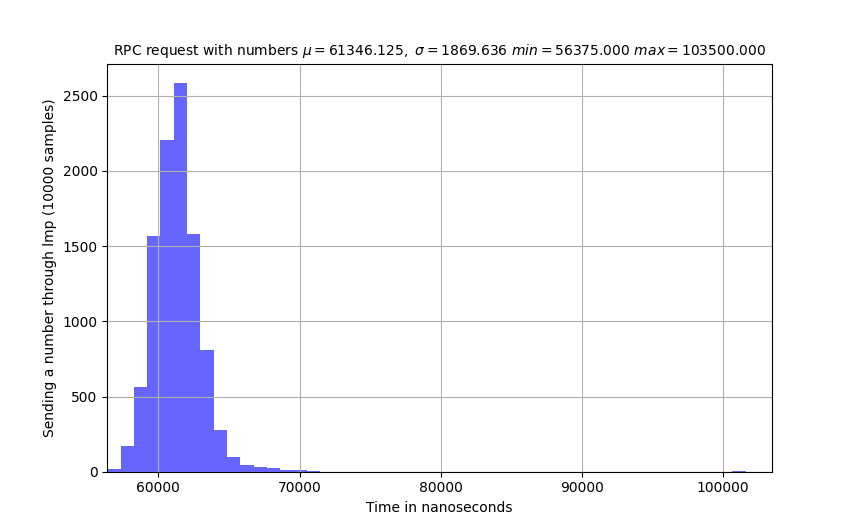
\includegraphics[width=12cm]{images/benchmarks/send_number.png}
    \caption{Latency to send a number over rpc}
    \label{fig:b1}
\end{figure}


\begin{figure}[htp]
    \centering
    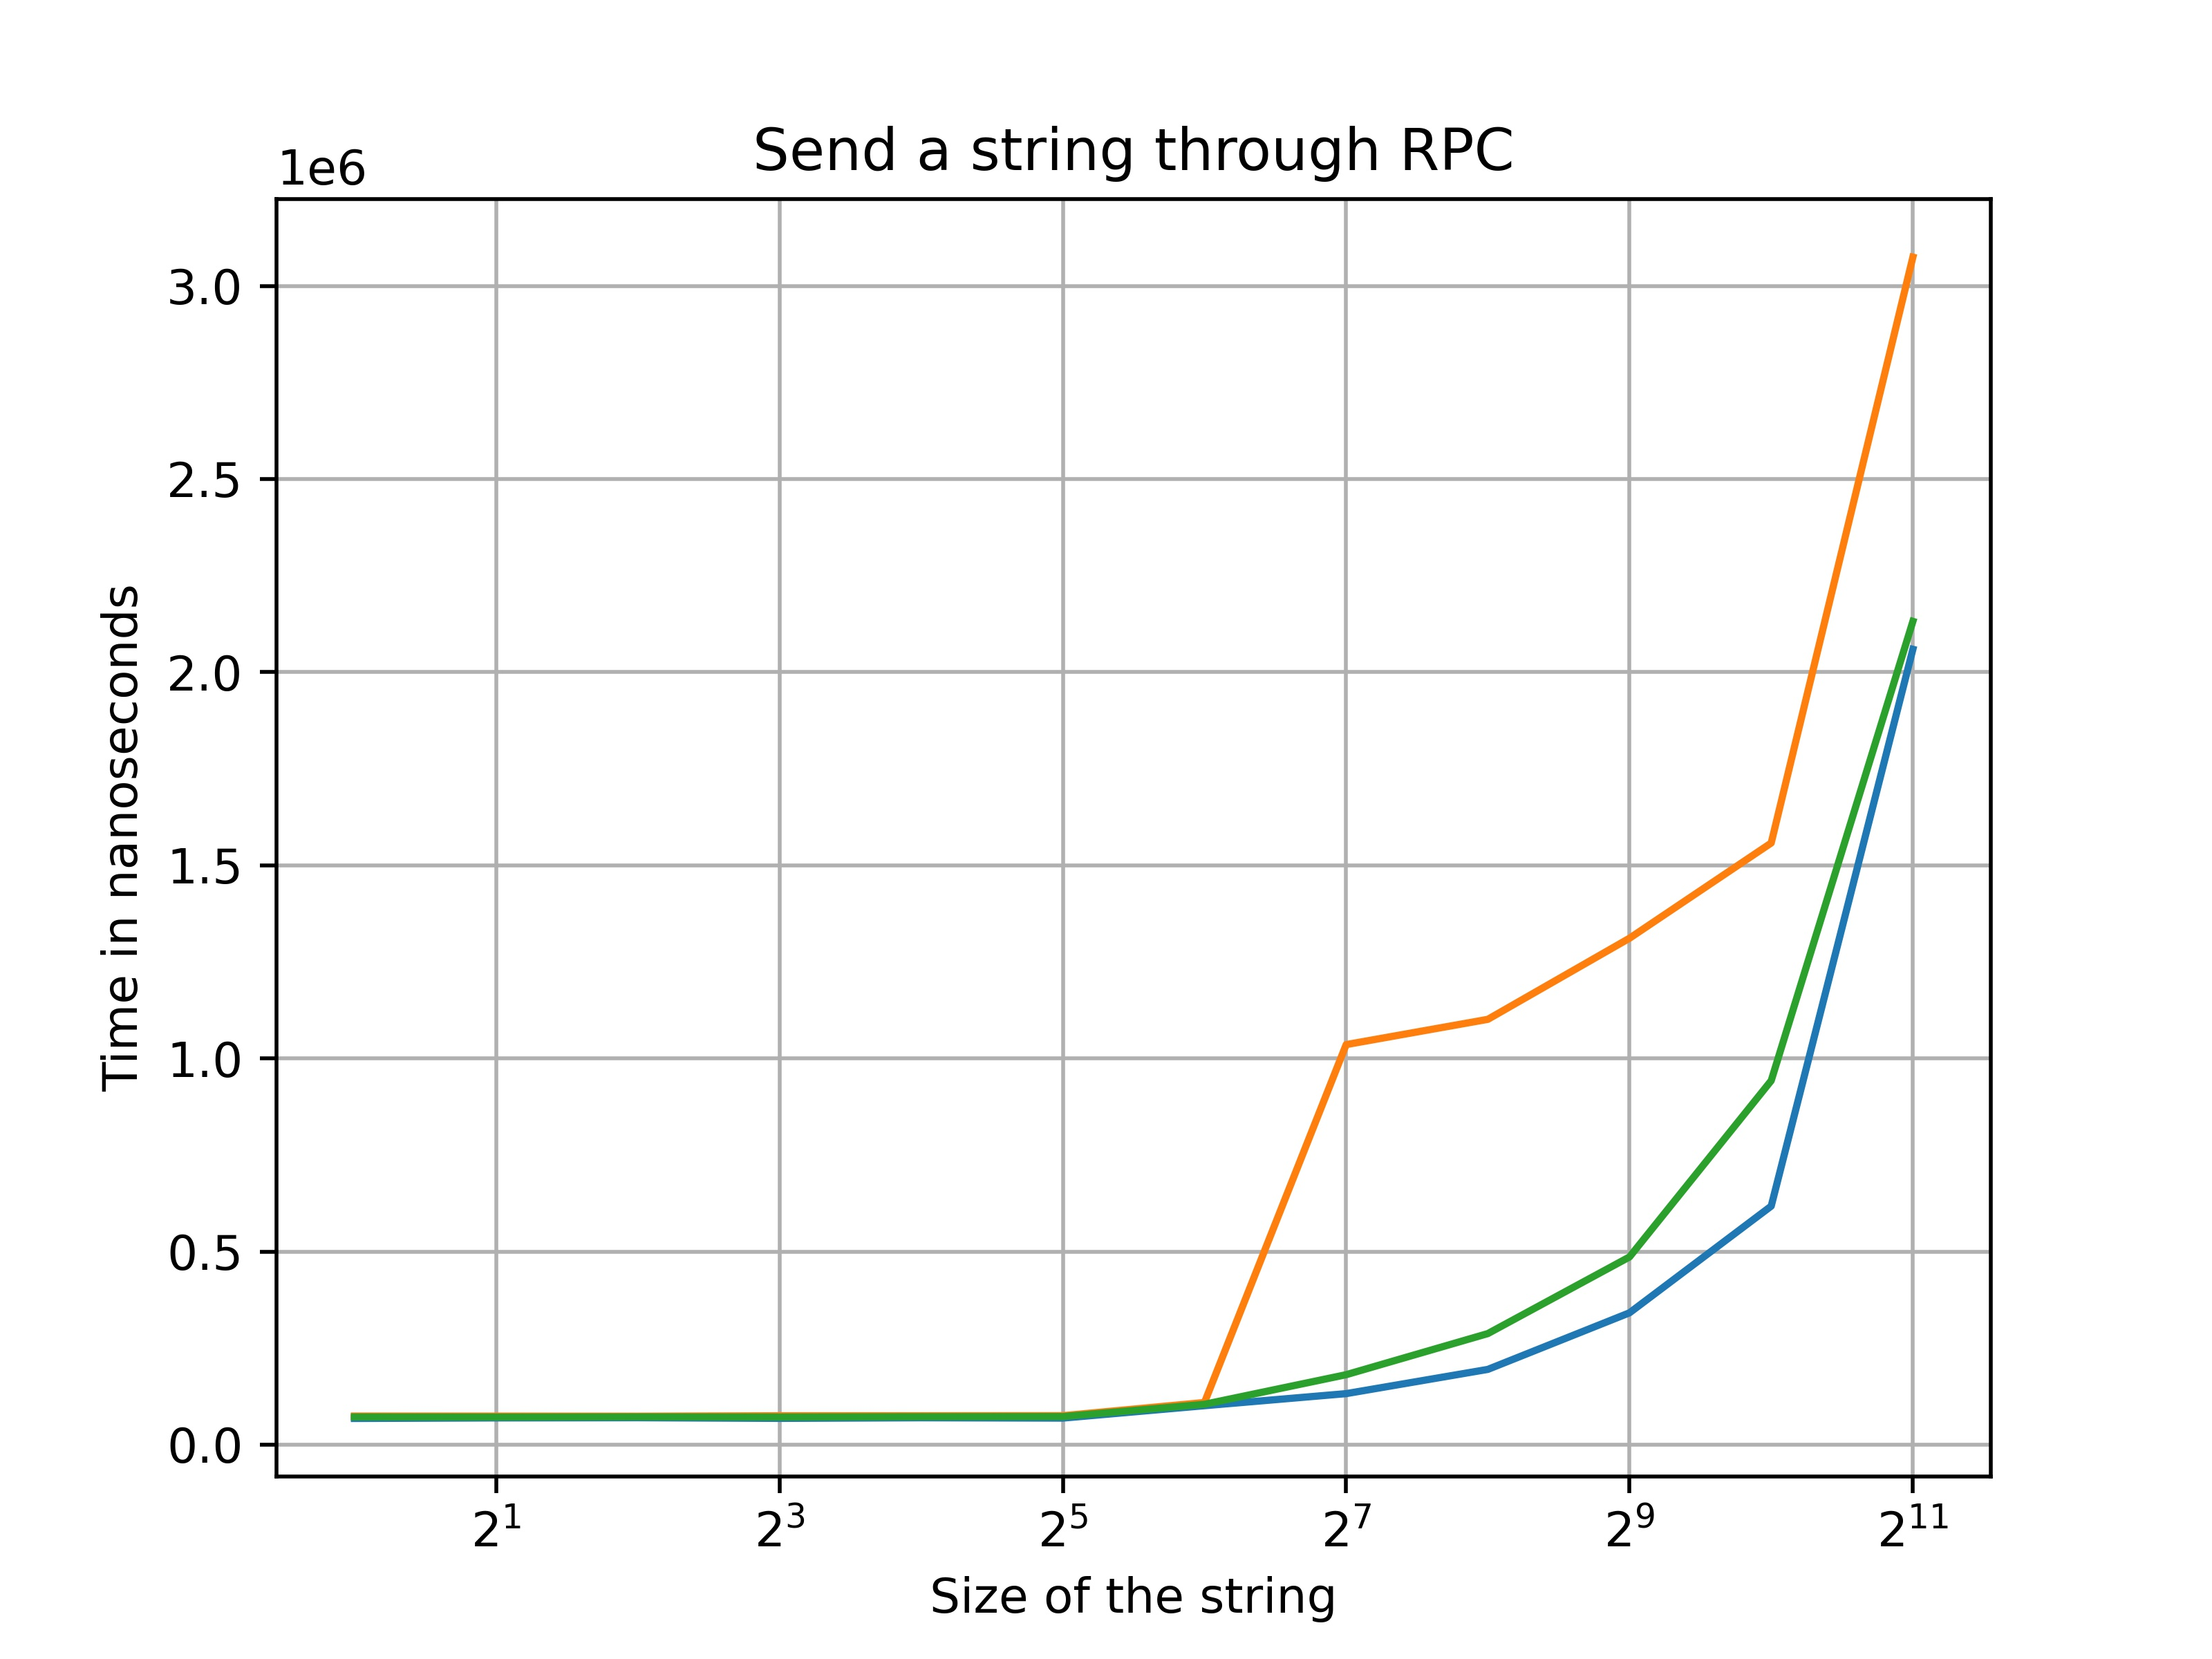
\includegraphics[width=12cm]{images/benchmarks/send_string.jpg}
    \caption{Latency to send a string over rpc}
    \label{fig:b2}
\end{figure}


\section{Measuring the physical memory allocator}

In this performance measurement, we are allocating 2560 pages of physical address without freeing any resource. The results clearly indicate that the performance gradually deteriorates over time. This decline in performance can be attributed to the necessity of traversing a linked list, which inherently takes a considerable amount of time. It is worth noting that these measurements are conducted on a newly initialized data structure, representing the optimal performance scenario. If we were to measure the performance when the data structure is not fresh, it would inevitably take more time as the performance worsens over time.

\begin{figure}[htp]
    \centering
    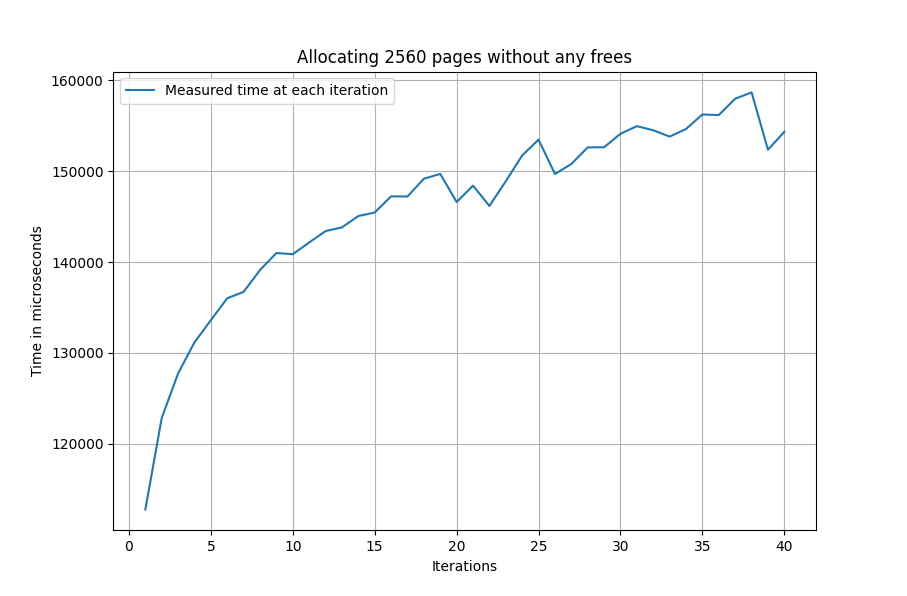
\includegraphics[width=12cm]{images/benchmarks/physical_allocator.png}
    \caption{Allocating multiple frames on the physical allocator}
    \label{fig:galaxy}
\end{figure}

\section{Measuring the virtual memory allocator}

In this  performance measurement, our focus lies on the allocation of virtual memory and the mapping of pages. It is crucial to note that in this particular benchmark, there is no actual measurement of physical allocation involved. Moreover, it is worth highlighting that our performance testing is conducted on a freshly established data structure. Just like in cases where physical memory is allocated, we observe a decline in performance as time progresses.

\begin{figure}[htp]
    \centering
    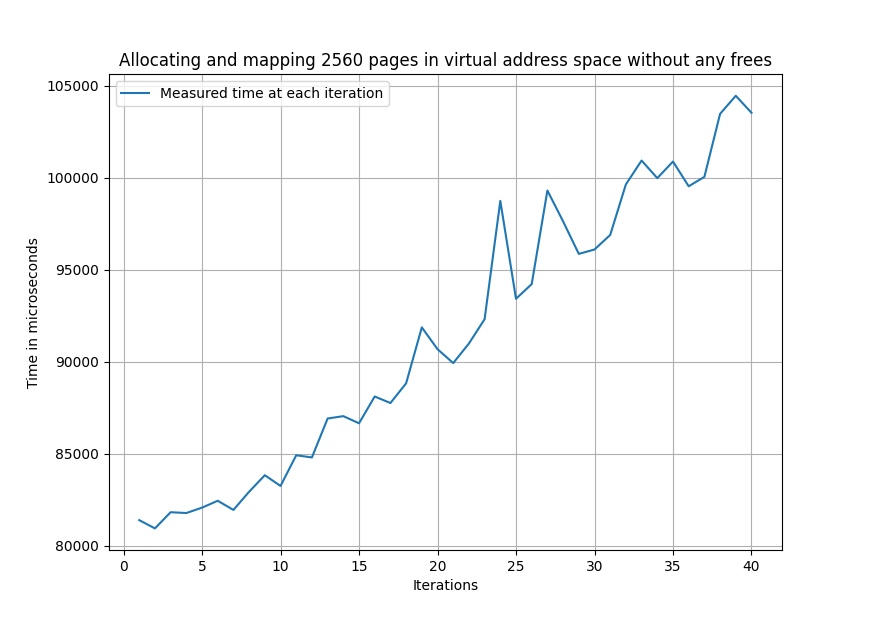
\includegraphics[width=12cm]{images/benchmarks/better.png}
    \caption{Allocating and mapping multiple frames on the virtual memory allocator}
    \label{fig:galaxy}
\end{figure}

\endgroup

\begingroup
\renewcommand\thechapter{C}
\chapter{Feedback}
{\normalfont\huge\bfseries}{}{}{\Huge}

The course was undeniably captivating and held our keen interest throughout its duration. We had the opportunity of delving into the intricate workings of operating systems and gained extensive knowledge in the process. Implementing an operating system from scratch provided us with a unique opportunity to comprehend its inner mechanisms. We encountered numerous trade-offs that necessitated careful consideration and decision-making. Furthermore, debugging proved to be more challenging in comparison to working on a single program.

\medskip

Another noteworthy positive aspect of the course that greatly enhanced our learning experience was working using a non-Unix kernel. This distinctive feature presented us with a valuable opportunity to engage in critical thinking regarding operating system designs. If we had been exposed only to a Unix-style operating system, the situation would likely have been quite different.
 
\medskip

On the whole, we express our heartfelt appreciation to the staff who orchestrated the course. The good organization ensured a smooth learning experience, and their regular presence and support on Moodle promptly addressed any concerns or difficulties we encountered.

\medskip

Nevertheless, one aspect of the course that warrants discussion is the workload. It is probably a recurring critique, but we feel compelled to highlight that the course's credit value of seven does not adequately reflect its intensity. Striking a balance between this course and our other academic commitments proved exceedingly hard, which is unfortunate. It is our belief that the course would be better served by being allocated 10-15 credits, as it would afford us more time to resolve bugs and align better with the significant investment of effort expected from students.

\endgroup